\documentclass[12pt]{article}

\usepackage[a4paper]{geometry}
\geometry{left=2.0cm,right=2.0cm,top=2.5cm,bottom=2.5cm}

\usepackage{ctex}

\usepackage[dvipsnames,svgnames]{xcolor}
\usepackage{tcolorbox}
\tcbuselibrary{skins}
\tcbuselibrary{minted}
\usemintedstyle{lovelace}
\usepackage{minted}

\usepackage{color}
\usepackage{tikz}
\usetikzlibrary{calc}
\usepackage{tabularx,colortbl}
\usepackage{amsfonts,amsmath,amssymb}
\usepackage{titling}
\usepackage{mathrsfs}
\usepackage{calc}
\usepackage{listings}

\usepackage[strict]{changepage} 
\usepackage{framed}
\definecolor{formalshade}{rgb}{0.95,0.95,1}
\usepackage{float}

\newenvironment{problem}[1]{
    \begin{prob}{#1}
}
{
    \tcblower
    \centering
    \textit{\scriptsize\bfseries Faculty Comments}
    \vspace{\baselineskip}
    \end{prob}
}

% 在此输入基本信息
\newcommand{\experiName}{边值问题的有限差分方法}
\newcommand{\advisorName}{童孝忠}
\newcommand{\studentName}{杨曜堃}
\newcommand{\studentNum}{8211221221}
\newcommand{\classNum}{地物2201班}

\begin{document}

\begin{center}
    ~\\
    ~\\
    \Huge \bf 《地球物理特殊方程》实验报告
\end{center}

\vspace{2.5cm}
\begin{figure}[htbp]
    \centering
    
\includegraphics[width=5.5cm]{Fig/logo.png}
\end{figure}

\vspace{4cm}
\begin{center}
    \Large \bf 班\qquad 级:\underline{\makebox[12em][c]{\kaishu \classNum}}

    \Large \bf 姓\qquad 名:\underline{\makebox[12em][c]{\kaishu \studentName}}

    \Large \bf 指导老师:\underline{\makebox[12em][c]{\kaishu \advisorName}}
\end{center}

\clearpage

\begin{center}
    \huge 实验一 \quad \experiName
\end{center}
\vspace{0.2cm}
\section{实验目的}
\begin{enumerate}
    \item 利用有限差分法求解一维Poisson方程的近似解,并设计MATLAB程序实现;
    \item 利用有限差分法求解二维Poisson方程定解问题;
    \item 编写MATLAB程序计算Neumann条件下二维Poisson方程的有限差分近似解。
\end{enumerate}
\section{实验内容}
\begin{description}
    \item[任务 1] 有限差分法求解下列问题并编写MATLAB程序\begin{equation*}
        \begin{cases}
            u''(x)=-\pi^2\sin(\pi x),\ 0<x<1\\
            u(0)=u(1)=0
        \end{cases}
    \end{equation*}其解析解为\begin{equation*}
        \color{blue}u(x)=\sin(\pi x)
    \end{equation*}
    \item[任务 2] 有限差分法求解下列问题并编写MATLAB程序\begin{equation*}
        \begin{cases}
            u''(x)=-\pi^2\sin(\pi x),\ 0<x<1\\
            u'(0)-u(0)=0.1,\ u(1)=0
        \end{cases}
    \end{equation*}其解析解为\begin{equation*}
        \color{blue}u(x)=\dfrac{1}{2}x^2-0.2x-0.3
    \end{equation*}
    \item[任务 3] 有限差分法求解下列问题并编写MATLAB程序\begin{equation*}
        \begin{cases}
            \dfrac{\partial^2u}{\partial x^2}+\dfrac{\partial^2u}{\partial y^2}=(1-\pi^2)e^x\sin(\pi y),\ &0<x<2,\ 0<y<1\\
            u(0,y)=\sin(\pi y),\ u(2,y)=e^2\sin(\pi y),\ &0\leqslant y\leqslant1\\
            u(x,0)=0,\ u(x,1)=0,\ &0\leqslant x\leqslant 2
        \end{cases}
    \end{equation*}其解析解为\begin{equation*}
        \color{blue}u(x,y)=e^x\sin(\pi y)
    \end{equation*}
    \item[任务 4] 有限差分法求解下列问题并编写MATLAB程序\begin{equation*}
        \begin{cases}
            \dfrac{\partial^2u}{\partial x^2}+\dfrac{\partial^2u}{\partial y^2}=-13\pi^2\sin\left(3\pi x+\dfrac{\pi}{4}\right)\sin\left(2\pi y+\dfrac{\pi}{4}\right),\ &0<x<1,\ 0<y<1\\
            \left.\dfrac{\partial u}{\partial x}\right|_{x=0}=3\pi\cos\left(\dfrac{\pi}{4}\right)\sin\left(2\pi y+\dfrac{\pi}{4}\right)&\\
            \left.\dfrac{\partial u}{\partial x}\right|_{x=1}=-3\pi\cos\left(\dfrac{\pi}{4}\right)\sin\left(2\pi y+\dfrac{\pi}{4}\right)&\\
            u|_{y=0}=\sin\left(\dfrac{\pi}{4}\right)\sin\left(3\pi x+\dfrac{\pi}{4}\right)&\\
            u|_{y=1}=\sin\left(\dfrac{\pi}{4}\right)\sin\left(3\pi x+\dfrac{\pi}{4}\right)
        \end{cases}
    \end{equation*}其解析解为\begin{equation*}
        \color{blue}u(x,y)=\sin\left(3\pi x+\dfrac{\pi}{4}\right)\sin\left(2\pi y+\dfrac{\pi}{4}\right)
    \end{equation*}
\end{description}

\newpage
\section{实验过程及结果}
对于任务1,编写MATLAB程序如下
\begin{tcblisting}{listing engine=minted,boxrule=0.1mm,
    colback=blue!5!white,colframe=blue!75!black,
    listing only,left=5mm,
    minted language=matlab,
    minted options={fontsize=\small,breaklines, autogobble,linenos,numbersep=3mm}}
clc;
clear;

X = 1;
N = 100;
dx = X/N;
x = 0:dx:X;

A = sparse(N+1,N+1);
b = zeros(N+1,1);

A(1,1) = 1;
A(N+1,N+1) = 1;
b(1,1) = 0;
b(N+1,1) = 0;
d = 1/dx^2;
for i = 2:N
    A(i,i) = -2*d;
    A(i,i-1) = d;
    A(i,i+1) = d;
    b(i,1) = -pi^2*sin(pi*i*dx);
end
u = A\b;

figure;
plot(x,u,'ro');
xlabel('x');
ylabel('u');
title('Ex1');    
\end{tcblisting}

\newpage
对于任务2,编写MATLAB程序如下
\begin{tcblisting}{listing engine=minted,boxrule=0.1mm,
    colback=blue!5!white,colframe=blue!75!black,
    listing only,left=5mm,
    minted language=matlab,
    minted options={fontsize=\small,breaklines, autogobble,linenos,numbersep=3mm}}
clc;
clear;

X = 1;
N = 100;
dx = X/N;
x = 0:dx:X;

A = sparse(N+1,N+1);
b = zeros(N+1,1);
A(1,1) = -1-dx;
A(1,2) = 1;
A(N+1,N+1) = 1;
b(1,1) = 0.1*dx;
b(N+1,1) = 0;
    
d = 1/dx^2;
for i = 2:N
    A(i,i) = -2*d;
    A(i,i-1) = d;
    A(i,i+1) = d;
    b(i,1) = 1;
 end
u = A\b;

figure;
plot(x,u,'ro');
xlabel('x');
ylabel('u');
title('Ex2');    
\end{tcblisting}

\newpage
针对任务3,编写MATLAB程序如下
\begin{tcblisting}{listing engine=minted,boxrule=0.1mm,
    colback=blue!5!white,colframe=blue!75!black,
    listing only,left=5mm,
    minted language=matlab,
    minted options={fontsize=\small,breaklines, autogobble,linenos,numbersep=3mm}}
clc;
clear;

X = 2;Y = 1;
N = 50;M = 50;
dx = X/N;dy = Y/M;
x = 0:dx:X;y = 0:dy:Y;

A = sparse((N+1)*(M+1),(N+1)*(M+1));
b = zeros((N+1)*(M+1),1);
p = 1/dx^2;q = 1/dy^2;
for i = 1:M+1
    for j = 1:N+1
        k = (j-1)*(M+1)+i;
        if(i==0||i==M+1)
            A(k,k) = 1;b(k,1) = 0;
        elseif(j==1)
            A(k,k) = 1;b(k,1) = sin(pi*i*dy);
        elseif(j==N+1)
            A(k,k) = 1;b(k,1) = exp(2)*sin(pi*i*dy);
        else
            A(k,k) = -2*p-2*q;A(k,k-1) = q;A(k,k+1) = q;
            A(k,k+(M+1)) = p;A(k,k-(M+1)) = p;
            b(k,1) = (1-pi^2)*exp(j*dx)*sin(pi*i*dy);
        end
    end 
end    
uij = A\b;
u = reshape(uij,M+1,N+1);

figure;
surf(x,y,u);
xlabel('x');
ylabel('y');
zlabel('u');
title('Ex3');
\end{tcblisting}

\newpage
针对任务4,编写MATLAB程序如下
\begin{tcblisting}{listing engine=minted,boxrule=0.1mm,
    colback=blue!5!white,colframe=blue!75!black,
    listing only,left=5mm,
    minted language=matlab,
    minted options={fontsize=\small,breaklines, autogobble,linenos,numbersep=3mm}}
clc;clear;

X = 1;Y = 1;
N = 50;M = 50;
dx = X/N;dy = Y/M;
x = 0:dx:X;y = 0:dy:Y;

A = sparse((N+1)*(M+1),(N+1)*(M+1));
b = zeros((N+1)*(M+1),1);p = 1/dx^2;q = 1/dy^2;
for i = 1:M+1
    for j = 1:N+1
    k = (j-1)*(M+1)+i;
        if(i==1)
            A(k,k) = 1;b(k,1) = sin(0.25*pi)*sin(3*pi*j*dx+0.25*pi);
        elseif(i==M+1)
            A(k,k) = 1;b(k,1) = sin(0.25*pi)*sin(3*pi*j*dx+0.25*pi);
        elseif(j==1)
            A(k,k) = -1;A(k,k+(M+1)) = 1;b(k,1) = 3*pi*cos(0.25*pi)*sin(2*pi*i*dy+0.25*pi)*dx;
        elseif(j==N+1)
            A(k,k) = -1;A(k,k-(M+1)) = 1;b(k,1) = -3*pi*cos(0.25*pi)*sin(2*pi*i*dy+0.25*pi)*dx;
        else
            A(k,k) = -2*p-2*q;A(k,k-1) = q;A(k,k+1) = q;
            A(k,k+(M+1)) = p;A(k,k-(M+1)) = p;
            b(k,1) = -13*pi^2*sin(3*pi*j*dx+0.25*pi)*sin(2*pi*i*dy+0.25*pi);
        end
    end 
end
uij = A\b;u = reshape(uij,M+1,N+1);

figure;
surf(x,y,u);
xlabel('x');ylabel('y');zlabel('u');
title('Ex4');
\end{tcblisting}

\begin{figure}[htbp]
    \small
    \centering
    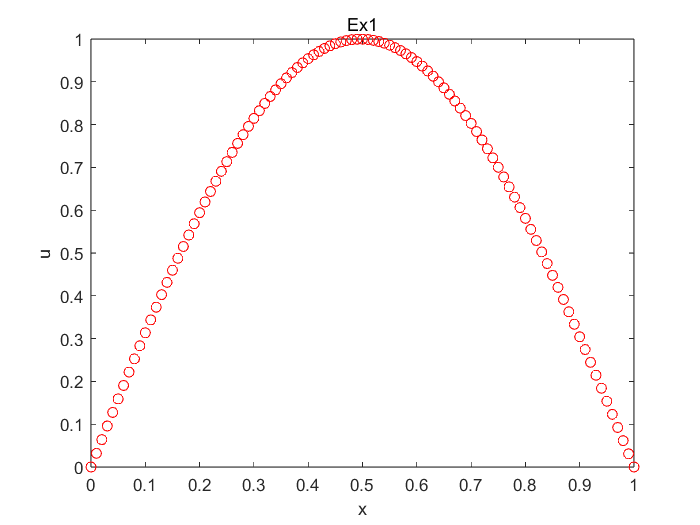
\includegraphics[width=6cm]{Fig/fig1.png}
    \caption{程序1运行结果}\label{fig1}
\end{figure}
\begin{figure}[htbp]
    \small
    \centering
    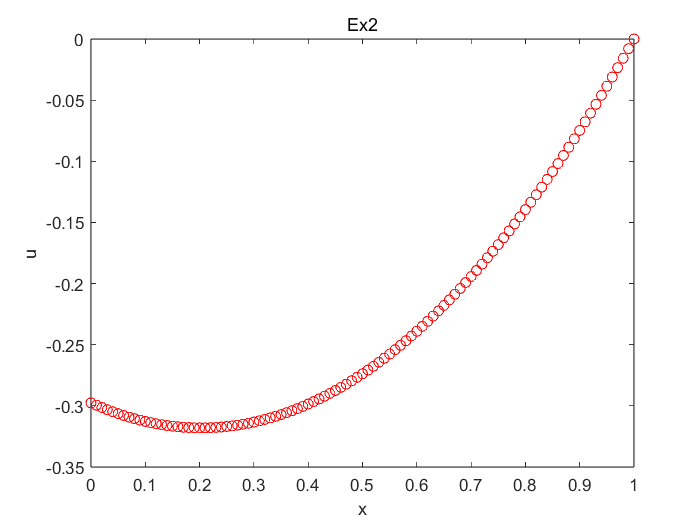
\includegraphics[width=6cm]{Fig/fig2.png}
    \caption{程序2运行结果}\label{fig2}
\end{figure}
\begin{figure}[htbp]
    \small
    \centering
    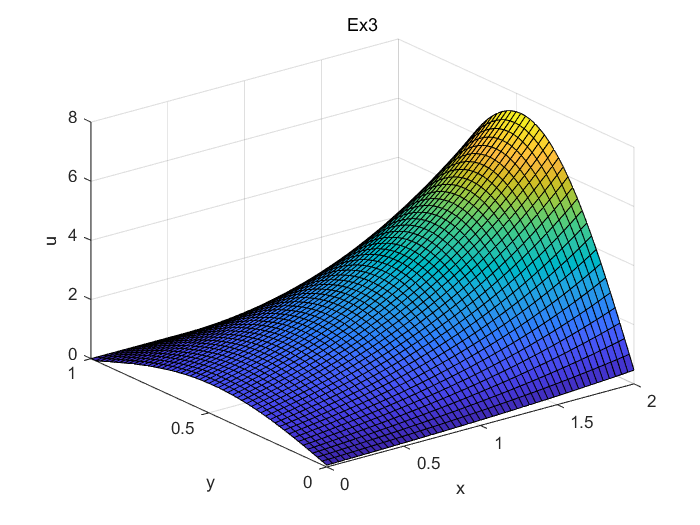
\includegraphics[width=6cm]{Fig/fig3.png}
    \caption{程序3运行结果}\label{fig3}
\end{figure}
\begin{figure}[htbp]
    \small
    \centering
    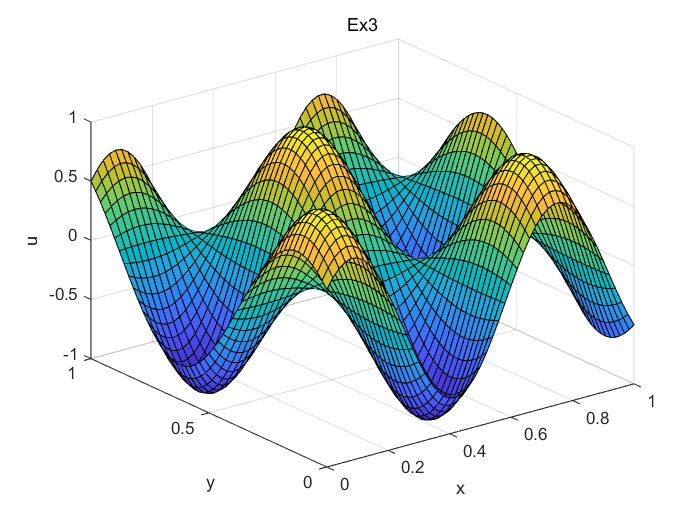
\includegraphics[width=6cm]{Fig/fig4.png}
    \caption{程序4运行结果}\label{fig4}
\end{figure}

\clearpage
\section{实验总结及收获}
\begin{enumerate}
    \item 学习了有限差分法求解一维二维Poisson方程;
    \item 学习了Neumann边界条件的有限差分法处理;
    \item 学习了MATLAB程序编写。
\end{enumerate}
\end{document}